\chapter{Estado del arte}
A continuación se explica a fondo la temática de este proyecto, así como sus posibles aplicaciones en la actualidad. 

\section{EMG}
La electromiografía se ha convertido en una de las técnicas más utilizadas en la actualidad para estudiar el potencial de acción de los músculos. Hacen uso de ella tanto neurofisiólogos, neurólogos y rehabilitadores. Se basa en la captación de las señales electromiográficas, las cuáles, son señales producidas por la musculatura a la hora de realizar una fase de contracción o relajación. Esta fase de contracción o relajación es producida por el estímulo de las motoneuronas. Existen dos tipos de motoneuronas. En este ámbito nos referimos a las motoneuronas somáticas que son las encargadas de las contracciones y relajaciones de la musculatura cuya acción es voluntaria.

Las motoneuronas forman parte de las unidades motoras (Figura \ref{fig:unidad motora}). Una unidad motora es realmente la encargada de las contracciones y relajaciones musculares y está formada por el conjunto de fibras musculares que afecta y la motoneurona encargada de enviar el estímulo. Cuando el impulso eléctrico de la motoneurona llega a las fibras musculares que afecta se obtiene un potencial de activación. El conjunto de todos los potenciales de activación de todas las fibras musculares que son activadas por una motoneurona se le conoce como el potencial de acción de la unidad motora. Lo que se analiza en la electromiografía es la actividad de las múltiples unidades motoras encargadas de un músculo \cite{konrad2005abc,suarez2013bases}.

\begin{figure}[ht]
\centering
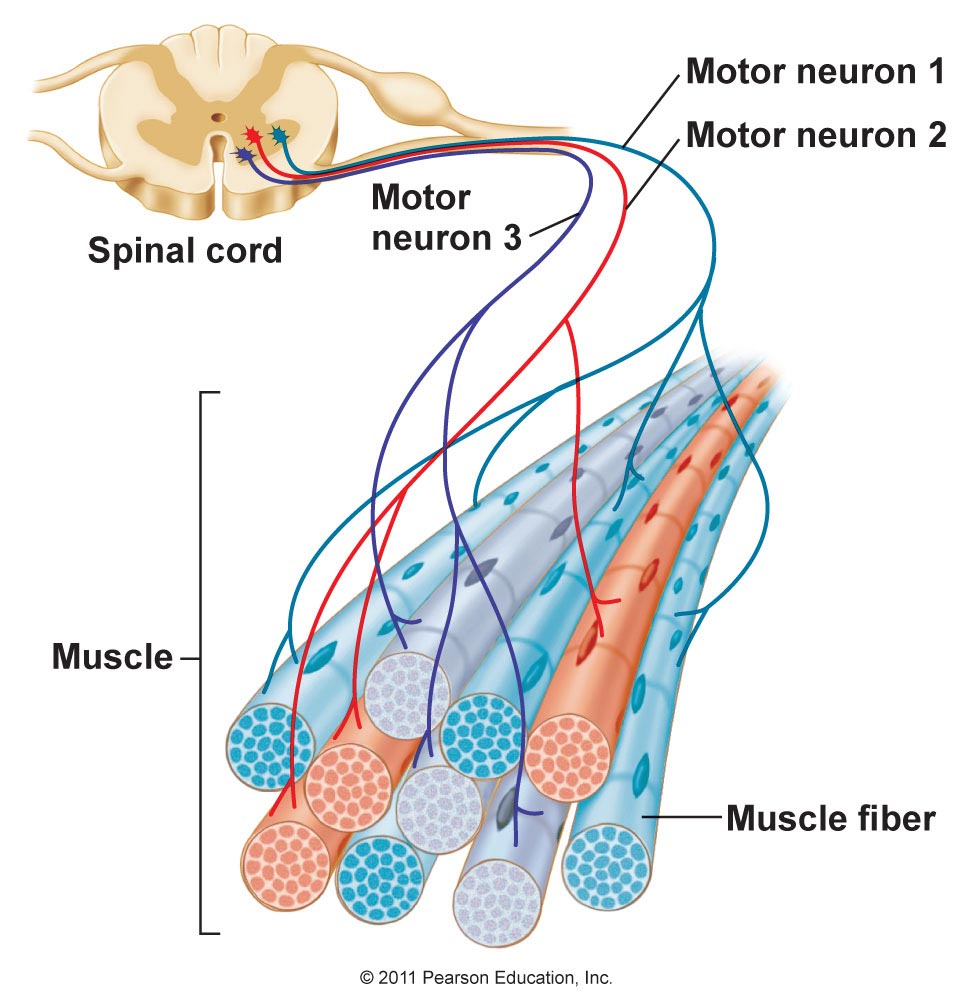
\includegraphics[scale=0.4]{imagenes/unidad motora.jpg}
\caption{Ejemplo de unidad motora \cite{unidadmotora}}
\label{fig:unidad motora}
\end{figure}

Estos impulsos eléctricos generados por las motoneuronas somáticas y que contraen o relajan el músculo son registrados en forma de señales electromiográficas y son utilizadas para ayudar a diagnosticar problemas de salud, que a simple vista, no pueden ser identificados. 

Para medir estas señales electromiográficas se pueden seguir dos métodos, el superficial y el intramuscular \cite{konrad2005abc}.

En la electromiografía intramuscular (Figura \ref{fig:intramuscular}), se utiliza una aguja electrodo para medir la actividad muscular. Esta aguja es introducida por la piel hasta llegar al músculo que queremos estudiar. Es mucho más precisa que la electromiografía de superficie, ya que al ser una aguja introducida directamente en el músculo, no recibe ruido externo de músculos adyacentes al estudiado. Por el contrario es más incomoda, ya que cada vez que se quiera hacer dicho análisis el paciente debe de ser pinchado, y puede que no esté dispuesto a dicho tratamiento. Además si se quiere analizar un actividad física compleja, como salto vertical, horizontal, carrera o sentadilla, como en el caso de este proyecto, el tener unas agujas introducidas en la musculatura puede ser molesto y hacer que la actividad física no se desarrolle a plenitud. Por último, para la utilización de esta técnica, se deberían de tener ciertos conocimientos médicos, ya que una persona sin dichos conocimientos no puede ser capaz de realizar el análisis de la forma correcta, al no conocer por ejemplo, el lugar óptimo para introducir la aguja. Otro agravante es que sin estos conocimientos, se podría llegar hasta la lesión del paciente, debido a introducir la aguja en el lugar no indicado. 

En la electromiografía de superficie (Figura \ref{fig:superficial}) se utilizan electrodos situados en la piel, que captan dichas señales electromiográficas. Es un método no invasivo y fácil de utilizar, donde solo es necesario tener el conocimiento de cual es el lugar óptimo para la colocación de los electrodos. Existen varios tipos de electrodos que serán explicados en el próximo apartado. En este proyecto se ha hecho uso de la electromiografía de superficie.


\begin{figure}[!ht]
\centering
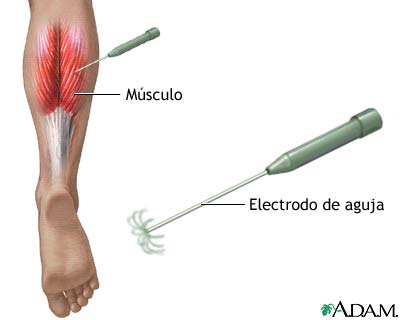
\includegraphics[scale=0.4]{imagenes/electrodo intramuscular.jpg}
\caption{Electromiografía intramuscular \cite{electrodoIntramuscular}}
\label{fig:intramuscular}
\end{figure}


\begin{figure}[!ht]
\centering
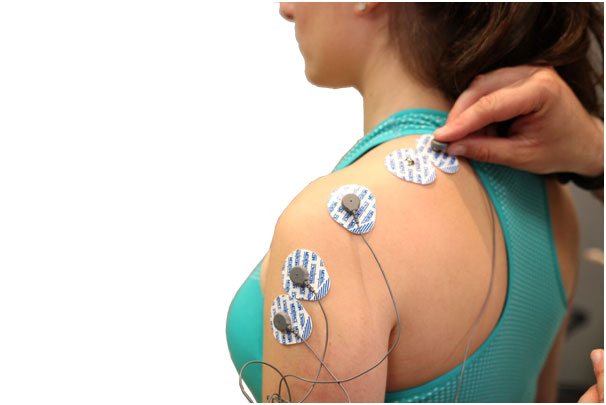
\includegraphics[scale=0.4]{imagenes/electrodo de superficie.jpg}
\caption{Electromiografía de superficie \cite{electrodoSuperficial}}
\label{fig:superficial}
\end{figure}



\subsubsection{EMG de superficie}
Para la realización de este proyecto se ha hecho uso de la electromiografía de superficie (EMGs). Esta técnica implica la utilización de electrodos situados en la piel, para la captación de las señales eléctricas. Por esto mismo, es necesario que en la mayoría de las ocasiones, para una mayor precisión en los datos tomados se realice una preparación de la piel en donde se van a situar los electrodos.

Por ejemplo, para que los electrodos queden mejor adheridos a la piel, a veces es necesario rasurar la piel para eliminar los pelos y que haya más superficie de contacto. También suele ser necesario limpiar la piel para eliminar partículas que dificulten la adherencia de los electrodos. Existen también electrodos que necesitan de la aplicación de un gel para su colocación, para así aumentar la precisión del electrodo. La funcionalidad de este gel es aumentar la conductividad entre la piel y el electrodo.

Otro factor importante es el tamaño del electrodo. Cuanto más pequeño sea, más precisión muscular nos dará, ya que, no cubrirá tanta superficie y no captará así actividad de músculos en los que no estamos interesados. El tamaño de los electrodos debería ser de 1 cm o menor \cite{konrad2005abc}.
\section{Aplicaciones médicas}
Como se ha comentado en secciones anteriores, el estudio de las señales de electromiografía es de gran utilidad para diagnosticar problemas motores y de salud. Algunas de estas enfermedades son: \cite{luzar2005electromiografia}
\begin{itemize}
\item Enfermedad de la neurona motora, ELA.
\item Radioculopatías, afectan a la columna vertebral, como por ejemplo, la ciática o la hernia de disco.
\item Plexopatías. Es difícil de conocer su origen. Produce un dolor y falta de movilidad en el brazo u hombro. Con el uso de la EMG intramuscular se puede llegar a conocer su origen.
\item Mononeuropatías agudas. Implican un daño en la medula espinal y produce hormigueo en la zona afectada.
\item Miopatía. Anomalía o mal funcionamiento en un grupo muscular, debido a un mal impulso eléctrico de las neuronas o a un mal funcionamiento del grupo muscular.
\end{itemize}

En este último punto va a ir centrado el proyecto, en facilitar el diagnostico de rodillas lesionadas a los fisioterapeutas que hagan uso de dicha herramienta. Para ello hace falta indagar en la base de la fatiga muscular y en que se ha basado el proyecto.

\section{Entrenamientos basados en velocidad y fatiga}
En la actualidad existe gran interés entre los atletas tanto profesionales como no profesionales, de mejorar su rendimiento. Para ello es indispensable pensar en un buen entrenamiento, ya que es la base de un buen rendimiento en la competición final. Para ello diversos estudios se han centrado en detectar la fatiga en los entrenamientos, ya que se considera, que entrenar bajo fatiga lo único que nos aporta es un lastre en el entrenamiento, ya que no reclutamos todas la unidades motoras necesarias y no se estimula lo suficiente al músculo. Además de que esto también supone un daño muy alto al sistema nervioso central.

Uno de los factores que indica la fatiga es la perdida de velocidad de ejecución en las actividades físicas, como por ejemplo, en las sentadillas. Se considera que una perdida del 20 por ciento en la velocidad de ejecución es indicativo de que existe una fatiga y por lo tanto se debe proceder a cortar la serie de entrenamiento y dar unos minutos de descanso para proseguir cuando el sujeto ya no esté sufriendo dicha fatiga \cite{fernandezpropuesta}.

Esta técnica dota al atleta de una gran capacidad de entrenamiento, ya que de dicha manera entrenará sin llegar a su limite y realizando siempre series efectivas, las cuáles, harán que se reclute el mayor número de unidades motoras y así obtener una mayor fuerza y desarrollo muscular. 

\section{Aplicación a este proyecto}

Como se ha explicado la electromiografía ha permitido grandes avances en la medicina y en el mundo del deporte. Este proyecto está más encaminado hacia los fisioterapeutas. Pretende desarrollar un sistema de clasificación, para que, sin la necesidad de medir la velocidad de ejecución de las series, se pueda determinar en el momento exacto de la prueba si el atleta está experimentando o no fatiga. Esto será de gran utilidad a atletas que quieran mejorar sus entrenamientos, así como, para que los fisioterapeutas obtengan más información, complementaria a los valores utilizados para la determinación de la actividad muscular como RMS, MNF, MDF, MAV, etc. 

Con toda esta información podrían llegar a conclusiones muy interesantes, tales como, en la ejecución de una sentadilla ver que músculos son los que entran en fatiga y determinar si se está produciendo una compensación muscular debido a una lesión de rodilla o por ejemplo, si dicho músculo está sufriendo algún tipo de daño y por ende su bajo rendimiento y fatiga tan temprana.
También puede ser utilizada para mejorar el rendimiento a la hora de entrenar, ya que detectaría la fatiga en tiempo real, y dotaría al atleta de una información real sobre su fatiga y así podría determinar si se necesita un descanso o por el contrario seguir realizando la actividad física.
